\documentclass[11pt]{article}
\usepackage{eacl2012}
\usepackage{times}
\usepackage{latexsym}
\usepackage{amsmath}
\usepackage{tikz}
\usepackage{graphicx}
\usepackage{multirow}
\usepackage{url}
\DeclareMathOperator*{\argmax}{arg\,max}
\setlength\titlebox{6.5cm}    % Expanding the titlebox

\title{Visualising Typological Relationships: Plotting WALS with Heat Maps}

 \author{Richard Littauer \\
 University of Saarland\\
 Computational Linguistics\\
 Saarbr\"ucken, Germany\\
   {\tt richard.littauer@gmail.com} \\\And
 Rory Turnbull \\
 Ohio State University\\
 Department of Linguistics\\
 Columbus, Ohio\\
   {\tt turnbull@ling.osu.edu} \\\AND
 Alexis Palmer\\
 University of Saarland\\
 Computational Linguistics\\
 Saarbr\"ucken, Germany\\
   {\tt apalmer@coli.uni-sb.de}\\} 

\date{}

\begin{document}
\maketitle

\begin{abstract}
This paper presents a novel way of visualising relationships between languages. The key feature of the visualisation is that it brings geographic, phylogenetic, and linguistic data together into a single image, allowing a new visual perspective on linguistic typology. The data presented here is extracted from the World Atlas of Language Structures (WALS)~\cite{wals-2011}. After pruning due to low coverage of WALS, we filter the typological data by geographical proximity in order to ascertain areal typological effects. The data are displayed in heat maps which reflect the strength of similarity between languages for different linguistic features. Finally, the heat maps are annotated for language family membership. The images so produced allow a multi-faceted perspective on the data which we hope will facilitate the interpretation of results and perhaps illuminate new areas of research in linguistic typology.
\end{abstract}

\section{Introduction}
This paper presents a novel %Should be fine - it is still novel
way of visualising relationships between languages. Relationships between languages can be understood with respect to linguistic features of the languages, their geographical proximity, and their status with respect to historical development. The visualisations presented in this paper are part of a new attempt %instead of the first time 
to bring together these three perspectives into a single image. One line of recent work brings computational methods to bear on the formation and use of large typological databases, often using sophisticated statistical techniques to discover relations between languages \cite[among others]{cysouw2011,daume07implication,daume09areal}, and another line of work uses typological data in natural language processing \cite[for example]{georgi:etal:10,lewis:xia:08}. The task of visually presenting the resulting data in this way has been only infrequently addressed. We are aware of some similar work \cite{mayer:etal:2010,rohrdantz:etal:2010} in visualising differences in linguistic typology, phylogeny \cite{multitree}% Fixed reference should be good now
, and geographical variation \cite{10.1371/journal.pone.0023613}. %Citing the Hong Kong paper, a couple of others.
 Here, we present our method for addressing the visualisation gap, bringing together phylogeny, typology, and geography %added for extra clarity
 by using data from the World Atlas of Language Structures \cite{wals-2011} to develop heat maps that can visually show the interconnected relationships between languages and language families. 

The main envisioned application of our visualisations is in the area of linguistic typology. Typology has been used to derive implications about possible languages, and about the ordering of the human mind. Different theorists have taken different views on the relationship between typology and the universality of languages. For example, Greenberg \shortcite{greenberg}, a foundational work, identified a number of cross-linguistic typological properties and implications and aimed to present them as truly universal -- relevant for \textit{all} languages. In a similar vein, typological universals have been employed as evidence in a generative story regarding language learning \cite{chomsky}.

Taking a different perspective, Dunn et al.\ \shortcite{Dunn_Greenhill_Levinson_Gray_2011} argued that a language's typology relies upon the previous generations' language more than on any biological, environmental or cognitive constraints, and that there are pathways which are generally followed in language change based on the previous parent language. What these arguments have in common is a reliance on a view of linguistic typology that is potentially restricted in its scope, due to insufficient access to broad-scale empirical data, covering many features of many languages of the world. 

The most comprehensive computational resource for linguistic typology currently available is the World Atlas of Language Structures (WALS).\footnote{As of 2008, WALS is browsable online (\url{http://www.wals.info}).}  WALS is a large database of details of structural properties of several thousand languages \cite{wals-2011}. The properties were collected from descriptive sources by the project's 55 authors.

However, of the 2,678 languages and 192 features in WALS, only 16\% of the possible data points are actually specified---the data are \emph{sparse}, and the sparsity of the data naturally makes it difficult to perform reliable statistical analysis. One way to work around this limitation is to seek meaningful visualisations of the data in WALS, instead of simply relying on raw numbers. This is our approach. 

In this paper, we first discuss in more detail the source data and the types of information extracted, followed by a discussion of some difficulties presented by the available data and our approaches for addressing those difficulties. Finally, we present a sample of the resulting visualisations.

\section{Aspects of the Visualisations}

The visualisations described here bring together three types of information: linguistic features, geographical distance, and phylogenetic distance. For the current study, all three types of information are extracted from the WALS database. In future work, we would explore alternate sources such as Ethnologue \cite{ethnologue} or MultiTree \shortcite{multitree} for alternate phylogenetic hierarchies. 

\subsection{Linguistic features}
At the time of writing, WALS contains information for 2,678 languages. The linguistic features covered in WALS range from phonetic and phonological features, over some lexical and morphological features, to syntactic structures, word order tendencies, and other structural phenomena. A total of 192 features are represented, grouped in 144 different chapters, with each chapter addressing a set of related features.  Ignoring the fact that a language having certain features will cancel out the possibility (or diminish the probability) of others, only 15.8\% of WALS is described fully. In other words, if we consider WALS to be a 2,678x192 grid, fewer than 16\% of the grid's squares contain feature values.

The coverage of features/chapters varies dramatically across languages, with an average of 28 feature values per language. The most populated feature has data for 1,519 languages. Because of the extreme sparsity of the data, we restricted our treatment to only languages with values for 30\% or more of the available features---372 languages, with a total of 36k feature values.

\subsection{Phylogenetic distance}

Languages are related phylogenetically either vertically, by lineage, or horizontally, by contact. In WALS, each language is placed in a tree hierarchy that specifies phylogenetic relations. In the WALS data files, this is specified by linking at three different levels: family, such as `Sino-Tibetan', sub-family, such as `Tibeto-Burman', and genus, such as `Northern Naga'. The WALS phylogenetic hierarchies do not take into account language contact. For that, we used geographic coordinates, which are present in WALS, as a proxy for contact. 

\subsection{Geographic distance}
Geographic distance is an important aspect of typological study because neighbouring  languages often come to share linguistic features, even in the absence of genetic relationship between the languages. Each language in WALS is associated with a geographical coordinate representing a central point for the main population of speakers of that language. We use these data to determine geographic distance between any two languages, using the haversine formula for orthodromic distance.\footnote{This measure is inexact, especially over long distances, due to the imperfect topography and non-spherical shape of the earth, but it is computationally simple and is accurate enough for our present purposes.}
%Haversine Formula - distance on a sphere (earth) http://en.wikipedia.org/wiki/Haversine_formula
% (Vincenty formula would be more accurate (as earth is not a 
% perfect sphere), but much more computationally intense for
% 2678*2678 comparisons.
%   http://www.codecodex.com/wiki/Calculate_Distance_Between_Two_Points_on_a_Globe#Python
%Note - reprint the data with this formula worked in, as it makes more sense than what you're doing at the moment.
A crucial aspect of our visualisations is that we produce them only for sets of languages within a reasonable geographic proximity and with sufficient feature coverage in WALS.

For this study, we used two approaches to clustering languages according to geographic distance. First, we chose an arbitrary radius in order to create a decision boundary for clustering neighbouring languages. For each language, that language's location is fixed as the centroid of the cluster and every language within the given radius is examined. We found that a radius of 500 kilometres provides a sufficient number of examples even after cleaning low-coverage languages from the WALS data. 

The second approach selected an arbitrary lower bound for the number of languages in the geographic area under consideration. If a sufficient percentage (enough to graph) of the total number of languages in the area remained after cleaning the WALS data, we took this as a useful area and did mapping for that area. This number is clearly under-representative of the amount of contact languages, as only half of the world's languages are present in WALS with any degree of coverage. This proxy was not as good as the radius method at choosing specific, useful examples for the \emph{n}-nearest neighbours, as the languages chosen were often quite distant from one another. 




\section{Heat Map Visualisations}

%We focus our visualisations on languages with a reasonable number of filled features, as drawing a heat map where only 16\%~of the features are available would be of little use. There are two options for dealing with this: to collapse the feature values in some way, or to select for languages that have a higher percentage of data filled than the average language. We opted for the second choice, and \emph{cleaned}  the file until it contained only languages that had at least 30\% as a lower bound of all of their entries filled. This cleaned data was then used in the other functions. 
We focused on producing visualisations only for features that are salient for the maximal number of selected languages. We choose two heat maps for display here, from the least sparse data available, to demonstrate the output of the visualisation method. The remaning visualizations, along with all code used to produce the visualisations, are avaliable in a public repository.\footnote{\url{https://github.com/RichardLitt/visualizing-language}}
%Added in this line to explain why we only have 2 graphs in here. 

All data was downloaded freely from WALS, all coding was done in either Python or R. The code was not computationally expensive to run, and the programming languages and methods are quite accessible. 

In a two-dimensional heat map, each cell of a matrix is filled with a colour representing that cell's value. In our case, the colour of the cell represents the normalised value of a linguistic feature according to WALS. Languages with the same colour in a given row have the same value for that typological feature.\footnote{Due to this reliance on colour, we strongly suggest viewing the heat maps presented here in colour.} Below we discuss two types of heat maps, focusing first on geographic and then on phylogenetic features.


\begin{figure}[!t]
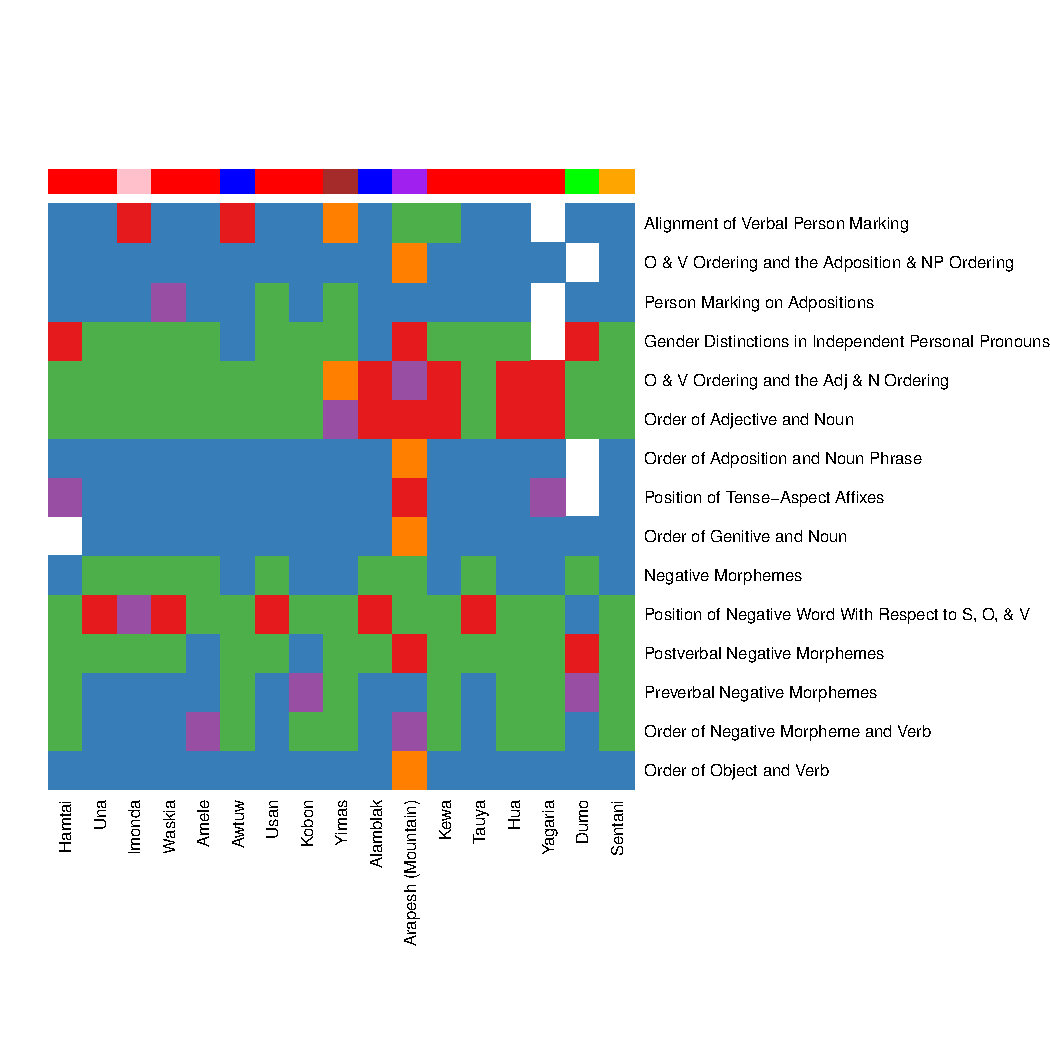
\includegraphics[width=3.1in]
{graph2yim.pdf} 
\caption{Geographically-focused heat map; see text for details. The bar at the top of the image represents the language family of the language in that column: Pink = Border; Red = Trans-New Guinea; Blue = Sepik; Brown = Lower Sepik-Ramu; Purple = Torricelli; Green = Skou; and Orange = Sentani.} 
\label{fig:heat1} 
\end{figure}


\subsection{Geographically-focused heat maps}
For the geographic distance maps, for each language present in the cleaned data, we identified all possible languages that lay within 500km, and sorted these languages until only the 16 closest neighbours were selected. Once the set of languages was determined, we selected for graphing only the most commonly-occurring features across that set of languages.
%We picked features to graph from among the resulting languages based on how common they were across the selected languages. 


To present the visualisation, we first centred the source language in the map. This decision was made in order to reduce the effect of one of the primary issues with using distance on a two dimensional graph; distance between two non-source languages is not shown, meaning that one could be to the north and another to the south. This means that the languages on the extremes of the map may be far apart from each other, and should be viewed with caution. %Does this work? Took out the egyptian example. 
%This issue the main justification for limiting the sphere of possible geographical languages to a %reasonable distance, given the data.


Figure~\ref{fig:heat1} shows a geographically-focused heat map with values for various morphological and word order features. The map is centred on Yimas, a language spoken in New Guinea. The features presented represent a particularly non-sparse section of WALS for this language area. A number of insights can be seen here. Most prominently, these languages are quite homogenous with respect to the selected features. Given that most of the languages do indeed belong to the same language family (cf. top bar of the graph), this is unlikely to be a chance effect.  In the 5th row (`O\&V Ordering and the Adj\&N Ordering'), we see via the cluster of red cells a partial grouping of languages close to Yimas, with less similarity at a greater distance. The nearly alternating pattern we see for `Position of Negative Word With Respect to S,O,\&V' may suggest areal groups that have been split by the data-centring function. Also, the checkerboard pattern for this feature and the one below (`Postverbal Negative Morphemes') suggests a possible negative correlation between these two linguistic features.


% The features were chosen based on their relative absence of missing data. For `Periphrastic Causative Constructions', the heat map shows partial grouping of languages closer to Yimas, and less similarity at a greater distance, as can be seen by the similar dark red features close to Yimas, but only orange at the extremes. The checkerboard pattern for dominant word orders may suggest groups that have been split by the data-centring function. In general, however, this graph shows that, for these features, the languages are for the most part homogenous. This is unlikely to be a chance effect, given the similarity in language families, as can be seen in the very top bar of the graph. Also, the checkerboard pattern for `Languages with 2 Dominant Orders of S, O, \& V' and `Multiple Negative Constructions in SVO Languages' suggests that the two corresponding WALS features avoid each other (have a negative correlation). 

\subsection{Phylogenetically-focused heat maps}

To produce phylogenetically-focused visualisations, for each language we identified other languages coming from the same family, subfamily, or genus. Figure~\ref{fig:heat2} shows a phylogenetically-focused heat map for Niger-Congo languages, arranged from west to east. A number of the western languages show red cells for features related to relative clauses; these can be compared to mostly blue cells in the eastern languages. We also see some apparent groupings for variable word order in negative clauses (red cells in western languages) and for NegSVO Order (purple cells in western languages). For some pairs of adjacent languages (most notably Bambara and Supyire), we see clusters of shared features. Especially give the importance of Bambara for 
%This example was chosen because the variance along the north-south access was optimally less than in other possible datasets. % Unsure about this sentence
syntactic argumentation \cite{culy}, this graph is an excellent example of visualisation pointing out an intriguing area for closer analysis.

%%% Rory, can you redo this graph so that it is from west to east? That would be more intuitive, wouldn't it? Instead of switching around the cardinal directions... Or is it already west to east?
% ==========
% It is already sorted west to east. -RJT %% Ok, changed the text to show this. 
% ==========

\begin{figure}[ht!]
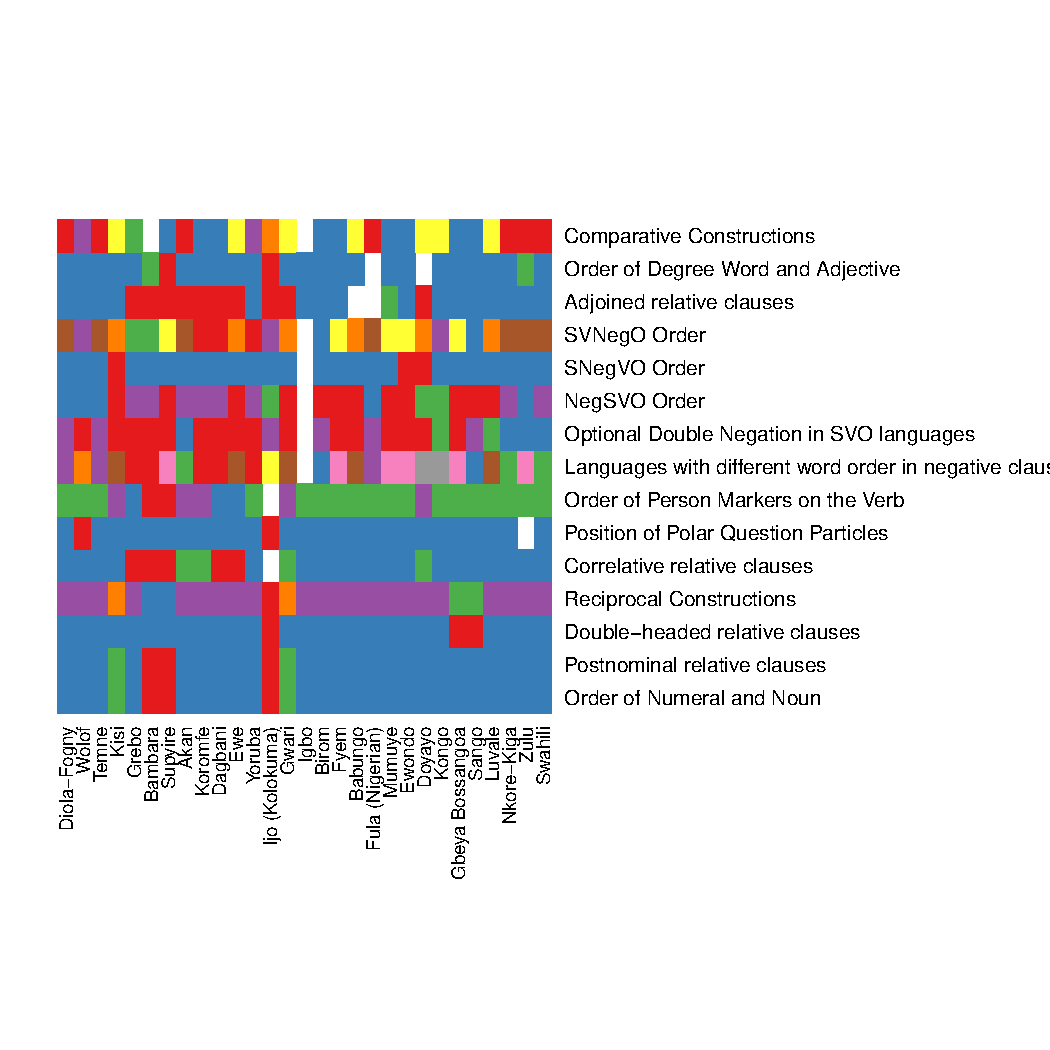
\includegraphics[width=3.1in]
{graph3nigercongo.pdf} 
\caption{Phylogenetic heat-map of Niger-Congo languages, arranged from west to east.} 
\label{fig:heat2} 
\end{figure}


%\subsection{Sparse data}
%
%\begin{figure}[h]
%\includegraphics[width=3.1in]
%{graph1sparsenew.pdf} 
%\caption{Scatterplot of language location (x and y axes), family (colour), and density of feature specification in WALS (size).} 
%\label{fig:sparse} 
%\end{figure}
%
%In Fig.~\ref{fig:sparse}, we have plotted out the neighbouring languages for the most populous language area represented on WALS by longitude and latitude. The centre language, Yimas, is a Trans-New Guinean language, and is the centre for the graph. The odd clustering is due to the Pacific Ocean--- such topographical features limit the usefulness of distance as a measure.  Another limit is the range of each language, which is not represented here, as each language is given only a single geographical coordinate that does not indicate the area over which the language resides, nor how many other languages coexist with it.
%
%For each language within 500km the number of features specified in WALS is shown. Only a small minority have more than 50\% of their features filled---there are only 171 such languages in WALS. This graph does not include languages not in WALS. 


\section{Conclusion}
In this paper we present a new approach to visualising relationships between languages, one which allows for the simultaneous viewing of linguistic features together with phylogenetic relationships and geographical location and proximity. These visualisations allow us to view language relationships in a multi-faceted way, seeking to work around the sparseness of available data and facilitate new insights into linguistic typology.

In this work we placed strong restrictions on both feature coverage and selection of salient features for representation, reducing the number of graphs produced to 6 with geographic focus and 8 with phylogenetic focus. One topic for future work is to explore other ways of working with and expanding the available data in order to access even more useful visualisations. In addition, it would be very interesting to apply this visualisation method to data from other sources, for example, data from multiple related dialects. In such cases, coverage is likely to be better, and the languages in question will have been selected already for their relatedness, thus avoiding some of the data-filtering issues that arise. Finally, we would like to investigate more principled approaches to selection, presentation, and ordering of linguistic features in the heat maps. 

\section*{Acknowledgments}
We are very grateful to the three anonymous reviewers for helpful comments on the current paper as well as many excellent ideas which will surely improve this work as we continue to develop it. 

\bibliographystyle{acl}
\bibliography{lingviz}

\end{document}


%==== Reviewer Comments ====
%I would recommend the authors not to write that these are the "first"
%visualizations that integrate geographical, phylogenetic, and typological data.
%At the ALT 2011 in Honkong there was a talk presenting a different
%visualization for the same purpose and there is further related research
%visualizing typological features in both phylogenetic context (e.g.
%http://multitree.linguistlist.org/) and with respect to geographical
%distributions, for example:
%
%%%%%I added the above reference in the intro, along with another one from the same group. We are still different in combining all of these, though. 


%- Nerbonne et al.: Gabmap - A Web Application for Dialectology.
%%%% Hard to find bibtex, found this: John Nerbonne, Rinke Colen, Charlotte Gooskens, Peter Kleiweg and Therese Leinonen
%Gabmap — A Web Application for Dialectology. Dialectologia. Special Issue II, (2011), pp.65-89. (Spec. Iss. Production, Perception and Attitude ed. by John Nerbonne, Stef Grondelaers, Dirk Speelman & Maria-Pilar Perea) 
%%%%hard to bibtexise...
%- Mayer et al.: Consonant co-occurrence in stems across languages: Automatic
%analysis and visualization of a phonotactic constraint.
%
%%%% We should perhaps state that these did separate work, such as just geographical distribution, or just phylogenetic content.
%
%Usually heat maps are applied to quantitative data. However, the WALS features are mostly ordinal or nominal. For nominal data a wrong impression might be
%given. Perceptionally, orange is closer to red than yellow is to red. The idea
%of a heatmap is that the color similarity reflects the data similarity. Yet, in
%the case of nominal data, colors should not have a perceptual ranking, because
%all categories are equally similar/dissimilar. Actually, in Figure 1 you chose
%a different color mapping for the language family, which is another nominal
%variable. You should handle the nominal data dimensions of the WALS data
%similarly.

%%%%% Rory, can you get this one?

%Consequently, I would also recommend to name the visualization "pixel map" or
%"dense pixel display" instead of "heat map" in order to stay consistent with
%the standard visualization terminology.
%
%%%% Not sure about this. I think this is probably still a heat map. We'd have to change the title of the piece. Alexis - would we be able to do that?
%
%============================================================================
%                           REVIEWER #2
%============================================================================
%
%
%---------------------------------------------------------------------------
%Reviewer's Scores
%---------------------------------------------------------------------------
%
%To what extent is the paper relevant to the workshop?: 4
%                Originality of the work: 3
%                     Technical accuracy: 2
% Reference to previous/related research: 3
%Presentation (clarity, overall organization): 3
%                                English: 4
%                             Acceptance: 2
%
%
%---------------------------------------------------------------------------
%Comments
%---------------------------------------------------------------------------
%
%Although I very much like the approach of the present paper, I have the
%impression that this is more some kind of preliminary draft that has to be
%developed further. At the current state, I don't see much convincing insight to
%be gained from the figures presented in the paper, though I see the potential.
%I urge the authors to think further on this path.
%
%%%% I think this will become more clear when I present it at the conference with a pointer and more graphs. Yes? R
%
%Figure 1: the ordering of the rows and columns seems rather arbitrary. There is
%a tradition to use standard clustering approaches to get the maximum regularity
%inside the heat map. Why is this approach not used here? (e.g. check the option
%of the R function "heat map()")
%
%%%% I am guess this is because of the nominal data? R
%
%============================================================================
%                           REVIEWER #3
%============================================================================
%
%
%---------------------------------------------------------------------------
%Reviewer's Scores
%---------------------------------------------------------------------------
%
%To what extent is the paper relevant to the workshop?: 5
%                Originality of the work: 2
%                     Technical accuracy: 3
% Reference to previous/related research: 3
%Presentation (clarity, overall organization): 4
%                                English: 5
%                             Acceptance: 3
%
%
%---------------------------------------------------------------------------
%Comments
%---------------------------------------------------------------------------
%

%%%% Alexis, maybe you could get this section? I think you're probably better at writing this than i would be. We could drop a hint about dialect data.
%
%The author is not very explicit about the actual goals of the visualization, though (what are "meaningful" visualizations?, p.2; 
%what sort of relationships can be viewed in a new way?, p.4). 
%But I can imagine that the combination of these features
%can be used to detect areal patterns (cases of contact situations). My biggest
%problem with the approach is that I don't really see the patterns that the
%author claims to see in the visualizations. Moreover, although this is mostly a
%problem of the sparse input data, the application of the current method to the
%WALS data with only 6 and 8 visualizations produced is rather restricted. Maybe
%other data sources (maybe dialect data with better coverage) would be more
%interesting to look at first.
%
%
%The idea to visualize linguistic features is not entirely novel, as the author
%claims several times in the paper. There is a recent approach by Mayer et al.
%(ALT talk in Hong Kong 2011), who had a similar objective in mind. Likewise,
%the use of heat maps does not introduce a new visualization method. Rather, the author employs a standard visualization method to language data.
%
%- Some of the details of the visualizations are not entirely clear to me. For
%instance, how are the languages arranged in the geographically-focused heat
%maps? According to their longitudes? Why not according to their latitudes?

%%%% Uh, we actually explain this. Was this guy reading the paper?

%Likewise, in the phylogenetically-focused heat map (isn't the ordering in Fig 2
%west-east, rather than from east to west as described in the paragraph above?).
%The author should indicate why longitudinal data is considered to be more
%important for the visualization.
%
%%%% Rory, could you get below?
%
%- I have problems finding the patterns that the author describes for the
%visualizations (even when viewing the visualization in color). At least, they
%are not obvious from the visualizations. It is hard to combine the genealogical
%information in Fig. 1 with the linguistic features that are plotted in the heat
%map. In addition, the color does not indicate how closely two languages are
%related, only if they are from the same or a different language family. As
%future work, I would strongly recommend to work on this aspect of the
%visualization.
%- It is mentioned that 15 closest neighbors are selected (p.3) for the
%visualization, yet in the figures there are 16 languages plus the central
%language.
%
%I would recommend including previous work on visualizing language data (e.g.,
%Nerbonne's or Goebl's work for dialect data where language features are plotted with their geographical information)
%
%%%% So, we should include Nerbonnés work on Gabmap %% Included one of his. 
